
% VLDB template version of 2020-08-03 enhances the ACM template, version 1.7.0:
% https://www.acm.org/publications/proceedings-template
% The ACM Latex guide provides further information about the ACM template

\documentclass[sigconf, nonacm]{acmart}
\usepackage{booktabs}

%% The following content must be adapted for the final version
% paper-specific
\newcommand\vldbdoi{XX.XX/XXX.XX}
\newcommand\vldbpages{XXX-XXX}
% issue-specific
\newcommand\vldbvolume{14}
\newcommand\vldbissue{1}
\newcommand\vldbyear{2020}
% should be fine as it is
\newcommand\vldbauthors{\authors}
\newcommand\vldbtitle{\shorttitle} 
% leave empty if no availability url should be set
\newcommand\vldbavailabilityurl{https://doi.org/10.5281/zenodo.10708876}
% whether page numbers should be shown or not, use 'plain' for review versions, 'empty' for camera ready
\newcommand\vldbpagestyle{plain} 

\begin{document}
\title{RepEng Project: An Approach for Schema Extraction of JSON and Extended JSON Document Collections}

%%
%% The "author" command and its associated commands are used to define the authors and their affiliations.
\author{Timur Garipov}
\affiliation{%
  \institution{The University of Passau}
  \streetaddress{Innstraße 41, 94032 Passau}
  \city{Passau}
  \state{Germany}
  \postcode{94032}
}
\email{garipo01@ads.uni-passau.de}

\maketitle

%%% do not modify the following VLDB block %%
%%% VLDB block start %%%
% \pagestyle{\vldbpagestyle}
% \begingroup\small\noindent\raggedright\textbf{PVLDB Reference Format:}\\
% \vldbauthors. \vldbtitle. PVLDB, \vldbvolume(\vldbissue): \vldbpages, \vldbyear.\\
% \href{https://doi.org/\vldbdoi}{doi:\vldbdoi}
% \endgroup
% \begingroup
% \renewcommand\thefootnote{}\footnote{\noindent
% This work is licensed under the Creative Commons BY-NC-ND 4.0 International License. Visit \url{https://creativecommons.org/licenses/by-nc-nd/4.0/} to view a copy of this license. For any use beyond those covered by this license, obtain permission by emailing \href{mailto:info@vldb.org}{info@vldb.org}. Copyright is held by the owner/author(s). Publication rights licensed to the VLDB Endowment. \\
% \raggedright Proceedings of the VLDB Endowment, Vol. \vldbvolume, No. \vldbissue\ %
% ISSN 2150-8097. \\
% \href{https://doi.org/\vldbdoi}{doi:\vldbdoi} \\
% }\addtocounter{footnote}{-1}\endgroup
%%% VLDB block end %%%

%%% do not modify the following VLDB block %%
%%% VLDB block start %%%
\ifdefempty{\vldbavailabilityurl}{}{
\vspace{.3cm}
\begingroup\small\noindent\raggedright\textbf{Artifact Availability:}\\
The source code, data, and/or other artifacts have been made available at \url{\vldbavailabilityurl}.
\endgroup
}
%%% VLDB block end %%%

\section{Introduction}

In the rapidly evolving field of data science and software engineering, the reproducibility of research results stands as a cornerstone of scientific integrity and validation. The paper "An Approach for Schema Extraction of JSON and Extended JSON Document Collections"~\cite{JsonSchemaDiscovery} introduces an innovative methodology for extracting schemas from JSON and Extended JSON document collections, a critical task in understanding and utilizing data efficiently in various applications.

This report provides a detailed account of the replication project, an attempt to reproduce the results of the above article using a robust and containerized environment. Replication efforts serve to confirm the claims of the original work, ensure continuity of knowledge, and provide a platform for further research and development in data structuring and analysis.

This package successfully reproduced the original schema extraction method for JSON documents, adhering to the procedures outlined in a previous study.

\section{Background}

The original work’s significance lies in its approach to systematically derive schemas from unstructured or semi-structured JSON documents, ubiquitous in today’s web and data-driven applications. By retrieving documents with simple and complex attributes mainly in JSON (\textit{JavaScript Object Notation}) or Extended JSON formats (~\cite{6106531} ~\cite{7592700}), the methodology aids in better data organization, error detection, and optimization of data storage and retrieval processes. Central to our reproduction effort is confirming the effectiveness and accuracy of schema extraction as presented in the original study, particularly in terms of its applicability to diverse JSON structures and its impact on improving data management practices.

This project is dedicated to accurately reconstructing the research environment within a Docker container. It effectively encapsulates the application, its dependencies, and the necessary scripts for the JSON and Extended JSON schema extraction process. It uses multiple containers - one for the application and one for the MongoDB in which JSON documents will be stored. This approach ensures that the reproduction attempt is conducted in an isolated and controlled environment, closely mimicking the original setup and thereby minimizing discrepancies attributable to environmental differences. 

Reproducing these findings is critical not only for validating the original results but also for setting a precedent for reliability and transparency in research methodologies in the field.


\section{Hypothesis and Research Questions}

In pursuit of validating the aforementioned paper, our study tests the following hypothesis: The methodology from the original study accurately and effectively extracts schemas from various unstructured or semi-structured JSON documents, enhancing data organization, error detection, and storage optimization.

\begin{table}[h!]
\centering
\caption{Original Paper ~\cite{JsonSchemaDiscovery} Table Featuring JSON Schema Extraction}
\label{tab:original-table}
\begin{footnotesize}
% \begin{tabular}{@{}lrrrrrr@{}}
\begin{tabular}{|l|c|c|c|c|}
\hline
\multicolumn{2}{|c|}{\textbf{Datasets}} & \multicolumn{2}{c|}{\textbf{JSON Schema Discovery}} & \textbf{Wang et al.} \cite{WangSchemaManagement}\\
\hline
\textbf{Collection} & \textbf{N\_JSON} & \textbf{RS} & \textbf{ROrd} & \textbf{FS} \\
\hline
drugs & 3662 & 2818 & 2818 & 2818 \\
\hline 
companies & 24367 & 21312 & 21312 & 21302 \\
\hline
movies & 30330 & 25140 & 25140 & 25137 \\
\hline
\end{tabular}
\end{footnotesize}
\smallskip
\footnotesize{N\_JSON - Number of JSON documents. RS - Raw schemas. ROrd - Raw schemas with ordered structure. FS - Final Schemas.}
\end{table}

These research questions could be established:
\begin{itemize}
    \item Effectiveness: Can we replicate the effective schema extraction as claimed in the original study?
    \item Accuracy: Does our reproduction affirm the accuracy levels of schema extraction reported in the original study?
    \item Applicability: Is the methodology consistently effective and accurate across diverse JSON document structures?
    \item Impact: How does schema extraction impact data management practices in our reproduction context?
\end{itemize}


In this report, the goal is to closely replicate the findings of the referenced paper using the tools and procedures outlined in the reproduction package. Table \ref{tab:original-table} shows the number of distinctly identified schemas from DBPedia datasets that were used by the work of Want et al. \cite{WangSchemaManagement} and by the work of Frozza et al. \cite{JsonSchemaDiscovery}

In this study, an MD5 checksum method is utilized to verify the accuracy of data schemas against originals. This approach helps identify whether recreated data aligns with the initial datasets. Small differences may arise due to various factors like file formats, but these are generally not significant. The primary objective is to ensure that critical aspects of the data remain consistent with original findings. If the MD5 checksums match, it signifies successful replication of data. This method ensures the reliability of results while allowing for minor, non-critical variations.


\section{Implementation}
This section outlines the environment setup for the replication experiment, details the procedures for comparing the results with those presented in the original paper, and includes a table summarizing the findings. It covers the technical environment configuration, step-by-step procedures adopted for the experiment, and detailed comparison protocols to align with the original study's outcomes.

\subsection{Environment}
The replication environment is configured using Docker containers, one hosting the original application for JSON Schema Discovery as detailed in the original paper \cite{JsonSchemaDiscovery}, and another for MongoDB. These are set up and managed using a docker-compose file to ensure they work seamlessly together.

In this reproduction study, the original codebase has been preserved without any modifications to maintain the integrity of the original application. Instead, additional Python code was developed to interact directly with the application's API, eliminating the need for a front-end interface. This modification allows for the entire evaluation process to be executed through a single command, \textit{"doAll.sh"}, streamlining the replication process.

It's important to note that the original research was conducted on the ASUS K45VM Notebook (Intel® Core™ i7 3610QM @ 2.30 GHz, 8GB RAM). In contrast, the replication experiments were performed on the MacBook Air M1 2020 (Apple M1 Chip, 16GB Memory). Despite the hardware differences, the results remained consistent between the two environments, largely because our comparison metrics, based on MD5 hash values, render time evaluation, and other hardware-dependent factors non-critical in our analysis.

\subsection{Experiment results}

\begin{table}
\centering
\caption{Comparison of Generated Schema Values from Reproduction Script Execution} \label{results-table}
\scalebox{0.80} {
\begin{tabular}{|l|c|c|c|c|c|}
\hline
\multicolumn{2}{|c|}{\textbf{Datasets}} & \multicolumn{2}{c|}{\textbf{JSON Schema Discovery}} &
\multicolumn{2}{c|}{\textbf{Frozza et al. \cite{JsonSchemaDiscovery}}} \\
\hline
\textbf{Collection} & \textbf{N\_JSON} & \textbf{RS} & \textbf{ROrd} & \textbf{RS} & \textbf{ROrd} \\
\hline
% Values will be generated here and replace 
%RESULT%

\end{tabular}
}

\end{table}

Table \ref{results-table} compares schema discovery outcomes obtained from this reproduction package against the results reported by Frozza et al. in their original study.

The table features two sections: 'Datasets', detailing the collection and number of JSON documents, and 'Comparison Sections', contrasting 'JSON Schema Discovery' (our results) with 'Frozza et al.' (original study), focusing on 'RS' (Raw Schemas) and 'ROrd' (Ordered Schemas).

This table layout, the same as used in the original paper for comparing with Wang et al., allows for an easy comparison between our results and Frozza et al.'s. It helps identify any similarities or differences in the schema discovery across various datasets.

% This comparative analysis demonstrates that the result from the current work align closely with those presented in the original paper. This alignment of results confirms the success of our reproduction, validating the reliability and reproducibility of the original findings. The consistent outcomes across different datasets further reinforce the robustness of the schema discovery process employed in the study.

\subsection{Verifying the accuracy of data schemas against originals}

\begin{figure}[H]
    \centering
    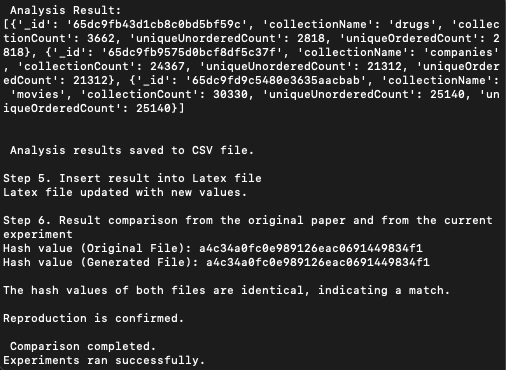
\includegraphics[width=\linewidth]{figures/analysis_result.png} 
    \caption{MD5 checksum comparison between original and reproduced data schemas.}
    \label{fig:md5_comparison}
\end{figure}

In this research, the MD5 checksum method was employed to ensure the accuracy of the reproduced data schemas against the originals. After the raw schema was extracted, the resulting data were saved into a CSV file. This CSV file was then subjected to a comparison against the original dataset's CSV file using the MD5 checksum approach. Figure \ref{fig:md5_comparison} illustrates the terminal output of the MD5 checksum comparison. The absence of differences between the checksums of the original and reproduced datasets verifies the accuracy of the replication process. This visual evidence complements our analytical findings, providing concrete proof that reproduction efforts have successfully mirrored the original study's outcomes.

\section{Limitations and threats to validity}

In this study, challenges were faced in validating reproduction results due to the original findings by Frozza et al. being available only in tabular format without accompanying JSON or CSV files. To enable direct comparison, a CSV file was manually created based on their Table 1 data, serving as a reference for reproduction despite format limitations.

\bibliographystyle{ACM-Reference-Format}
\bibliography{literature}

\end{document}
